
\chapter[Related Works]{Related Works}
\graphicspath{ {images/stateOfArt} }

\section{History of software visualization}

Essential parts of software lifecycles are software maintenance and software evolution. Both activities require the comprehension of the system by the developer. Mayrhauser \cite{VonMayrhauser1995} defined program comprehension as a process that uses knowledge to acquire new knowledge. Generally, programmers possess two types of knowledge: general knowledge and software-specific knowledge, which represent their level of understanding of that software. Software comprehension aims to increase this specific knowledge of systems, and, to do that, it can leverage some software visualization techniques. Software visualization supports the understanding of software systems because it enables the visualization of the system's information (architecture, source code, behavior) with a 2D or 3D representation. Stasko et al.\cite{Stasko2008} conducted a study in 1998 that shows how visualization arguments human memory since it works as external cognitive aid and thus, improves thinking and analysis capabilities. \\

Software visualization supports the understanding of software systems because it enables the visualization of the system's information (architecture, source code, behavior) with a 2D or 3D representation. Stasko et al.\cite{Stasko2008} conducted a study in 1998 that shows how visualization arguments human memory since it works as external cognitive aid and thus, improves thinking and analysis capabilitiesSoftware visualization supports the understanding of software systems because it enables the visualization of the system's information (architecture, source code, behavior) with a 2D or 3D representation. Stasko et al.\cite{Stasko2008} conducted a study in 1998 that shows how visualization arguments human memory since it works as external cognitive aid and thus, improves thinking and analysis capabilitiesow visualization arguments human memory since it works as external cognitive aid and thus, improves thinking and analysis capabilitiesSoftware visualization supports the understanding of software systems because it enables the visualization of the system's information (architecture, source code, behavior) with a 2D or 3D representation. Stasko et al.\cite{Stasko2008} conducted a study in 1998 that shows how visualization arguments human memory since it works as external cognitive aid and thus, improves thinking and analysis capabilities


\newpage
In the same year, Chuah and Erick \cite{Chuah1998} proposed three different techniques to visualize project data. They exploited the concept of glyphs, a graphical object that represents data through visual parameters. The first technique was the Timewhell glyph, used to visualize time-oriented information (number of lines of code, number of errors, number of added lines). The second technique was the 3D wheel glyph; it encoded the same attributes of the time wheel, and additionally, it used the height to encode time. Infobug glyph was the last technique, where each glyph was composed of four parts, each representing essential data of the system (time, code size, number of lines of code added/deleted/modified). \newline

\begin{figure}[H]
\minipage{0.32\textwidth}
  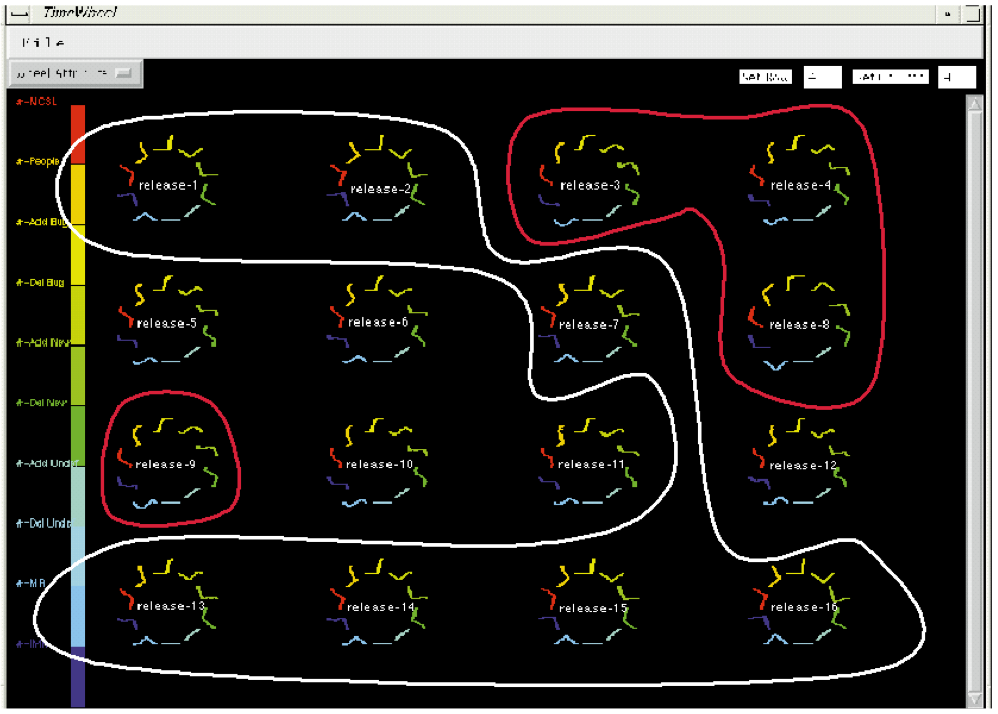
\includegraphics[width=\linewidth]{Chuan1.png}
  \caption{Timewhell}
\endminipage\hfill
\minipage{0.32\textwidth}
  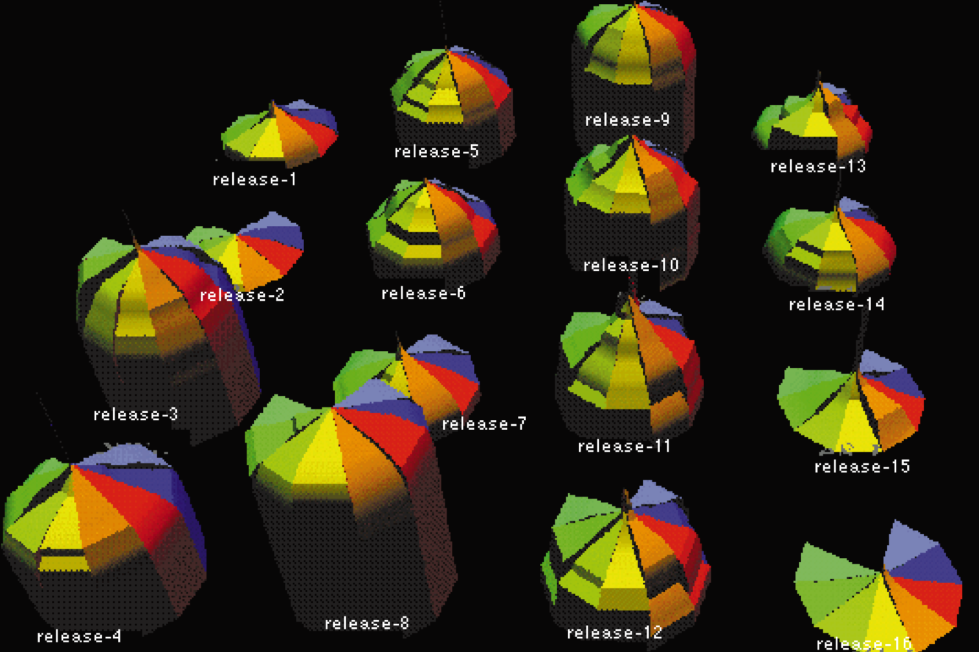
\includegraphics[width=\linewidth]{Chuan2.png}
  \caption{3D wheel}
\endminipage\hfill
\minipage{0.32\textwidth}%
  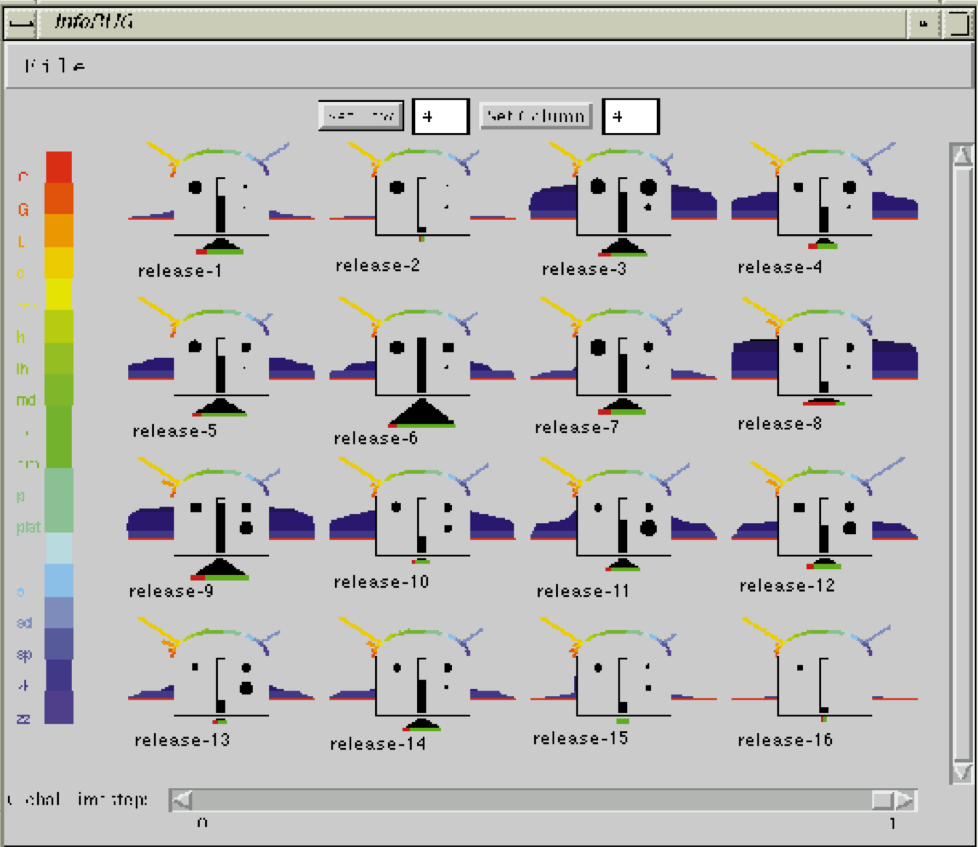
\includegraphics[width=\linewidth]{Chuan3.png}
  \caption{Infobug}
\endminipage
\end{figure}


In 2001 Lanza \cite{Lanza2001} introduced the concept of the Evolution Matrix. It was a way to visualize the evolution of software without dealing with a large amount of complex data. Furthermore, that approach was agnostic to any particular programming language. The Evolution Matrix aimed to display the evolution of classes in object-oriented software systems. Each column represented a version of the software, and each row represented a different version of the same class. The cells were filled with boxes whose size depended on two different metrics. Thanks to this approach, he was able to infer some evolution information by just looking at the shape of the matrix

\begin{figure}[H]
\minipage{0.49\textwidth}
  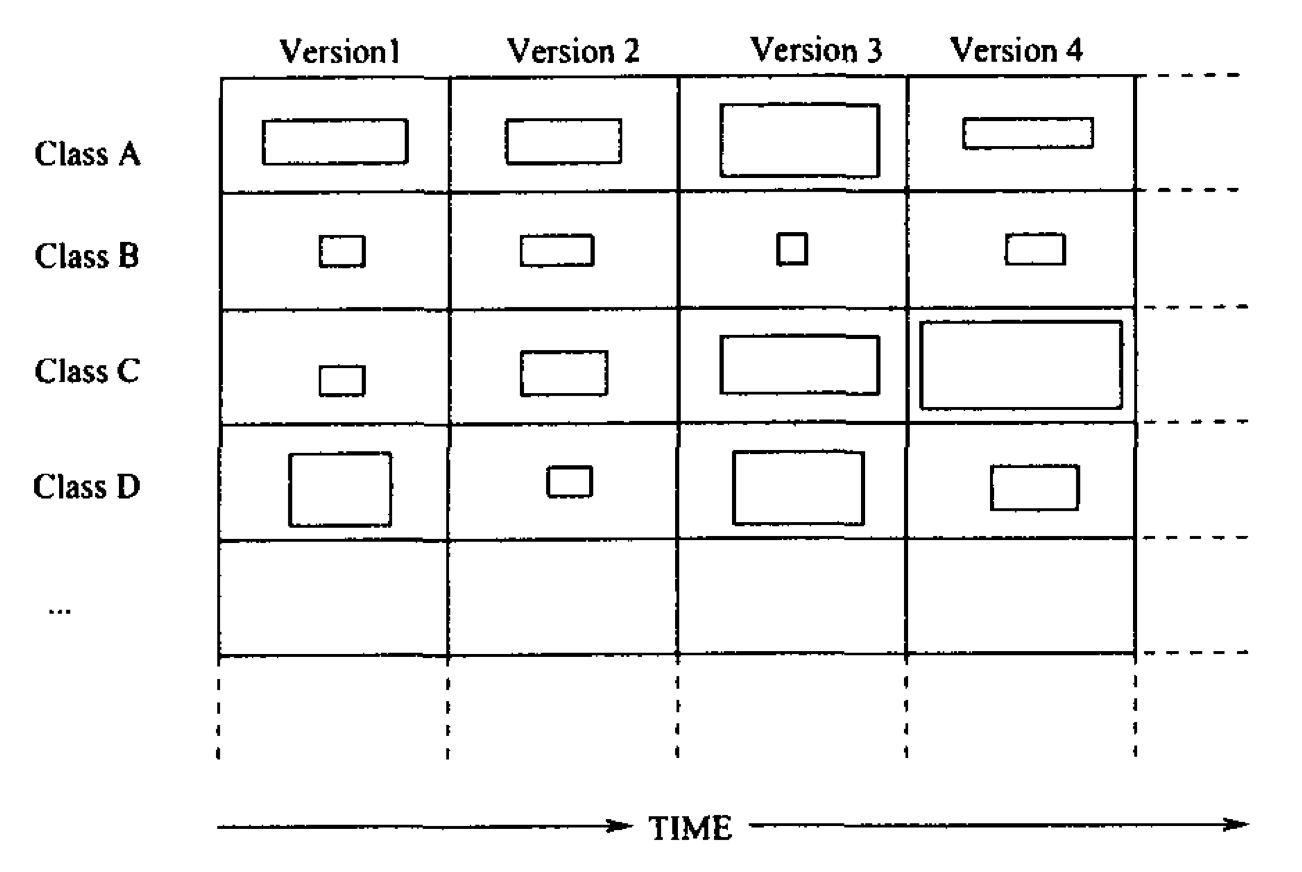
\includegraphics[width=\linewidth]{EvolutionMatrix1.png}
  \caption{A schematic display of the Evolution Matrix}
\endminipage\hfill
\minipage{0.49\textwidth}
  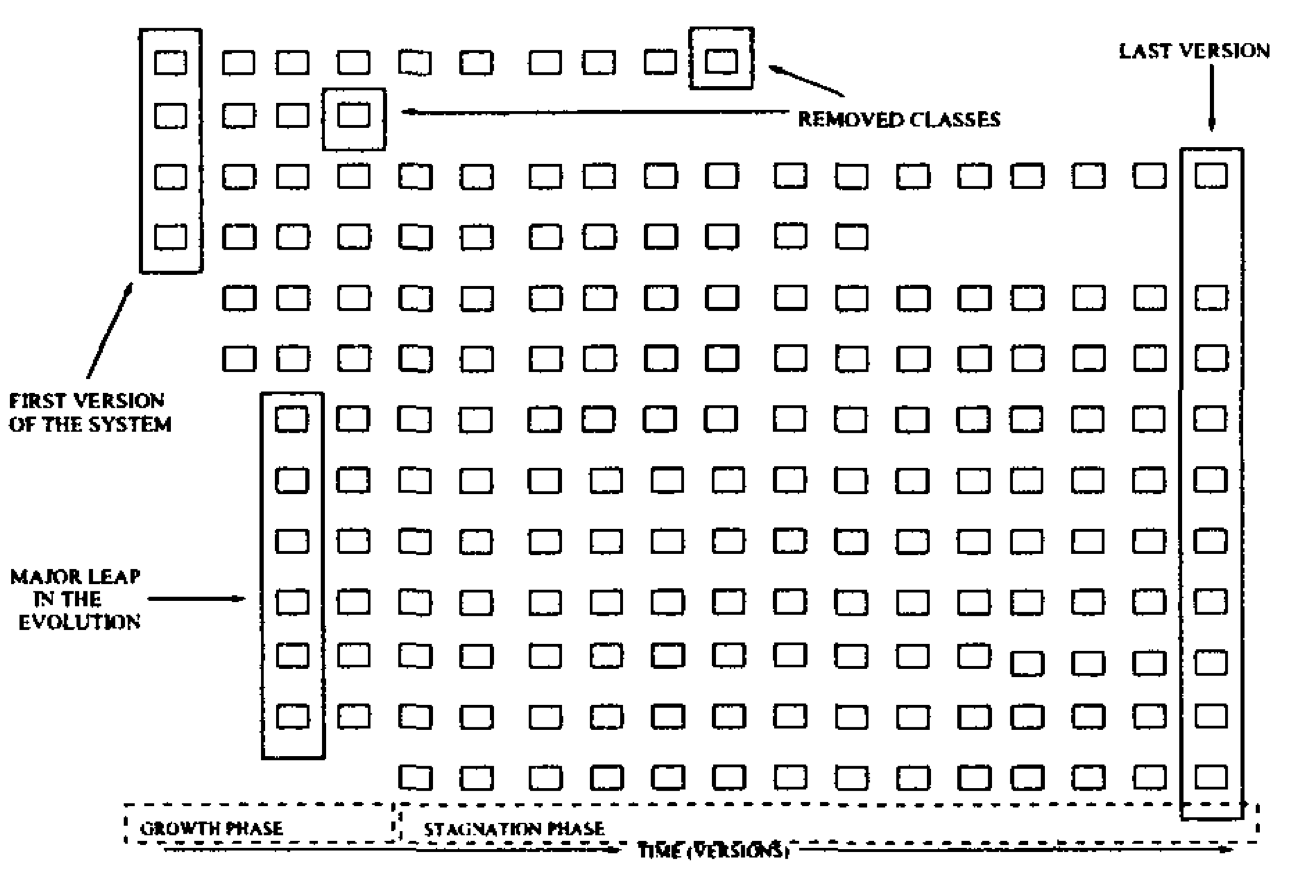
\includegraphics[width=\linewidth]{EvolutionMatrix2.png}
  \caption{Some characteristics of the Evolution Matrix}
\endminipage\hfill
\end{figure}

\newpage

Wettel in his thesis \cite{Wettel2011}, defined a city metaphor for software visualization that represents software as cities. His work represents packages as districts and classes as buildings. This metaphor was applied in different contexts related to reverse engineering (program comprehension, software evolution, software quality) to demonstrate metaphor's versatility. As a result, he found evidence that his approach works. However, he claims that city metaphor brings visual and layout limitations (not all visualization techniques fit well with it). Under those circumstances, he preferred simplicity over the accuracy, so he obtained a simple visual language that facilitates comprehension of data. He conducted an experiment of the evidence that the city metaphor enables the creation of efficient software visualizations. His approach was implemented by a software visualization tool called CodeCity that supports the city metaphor. 
\\
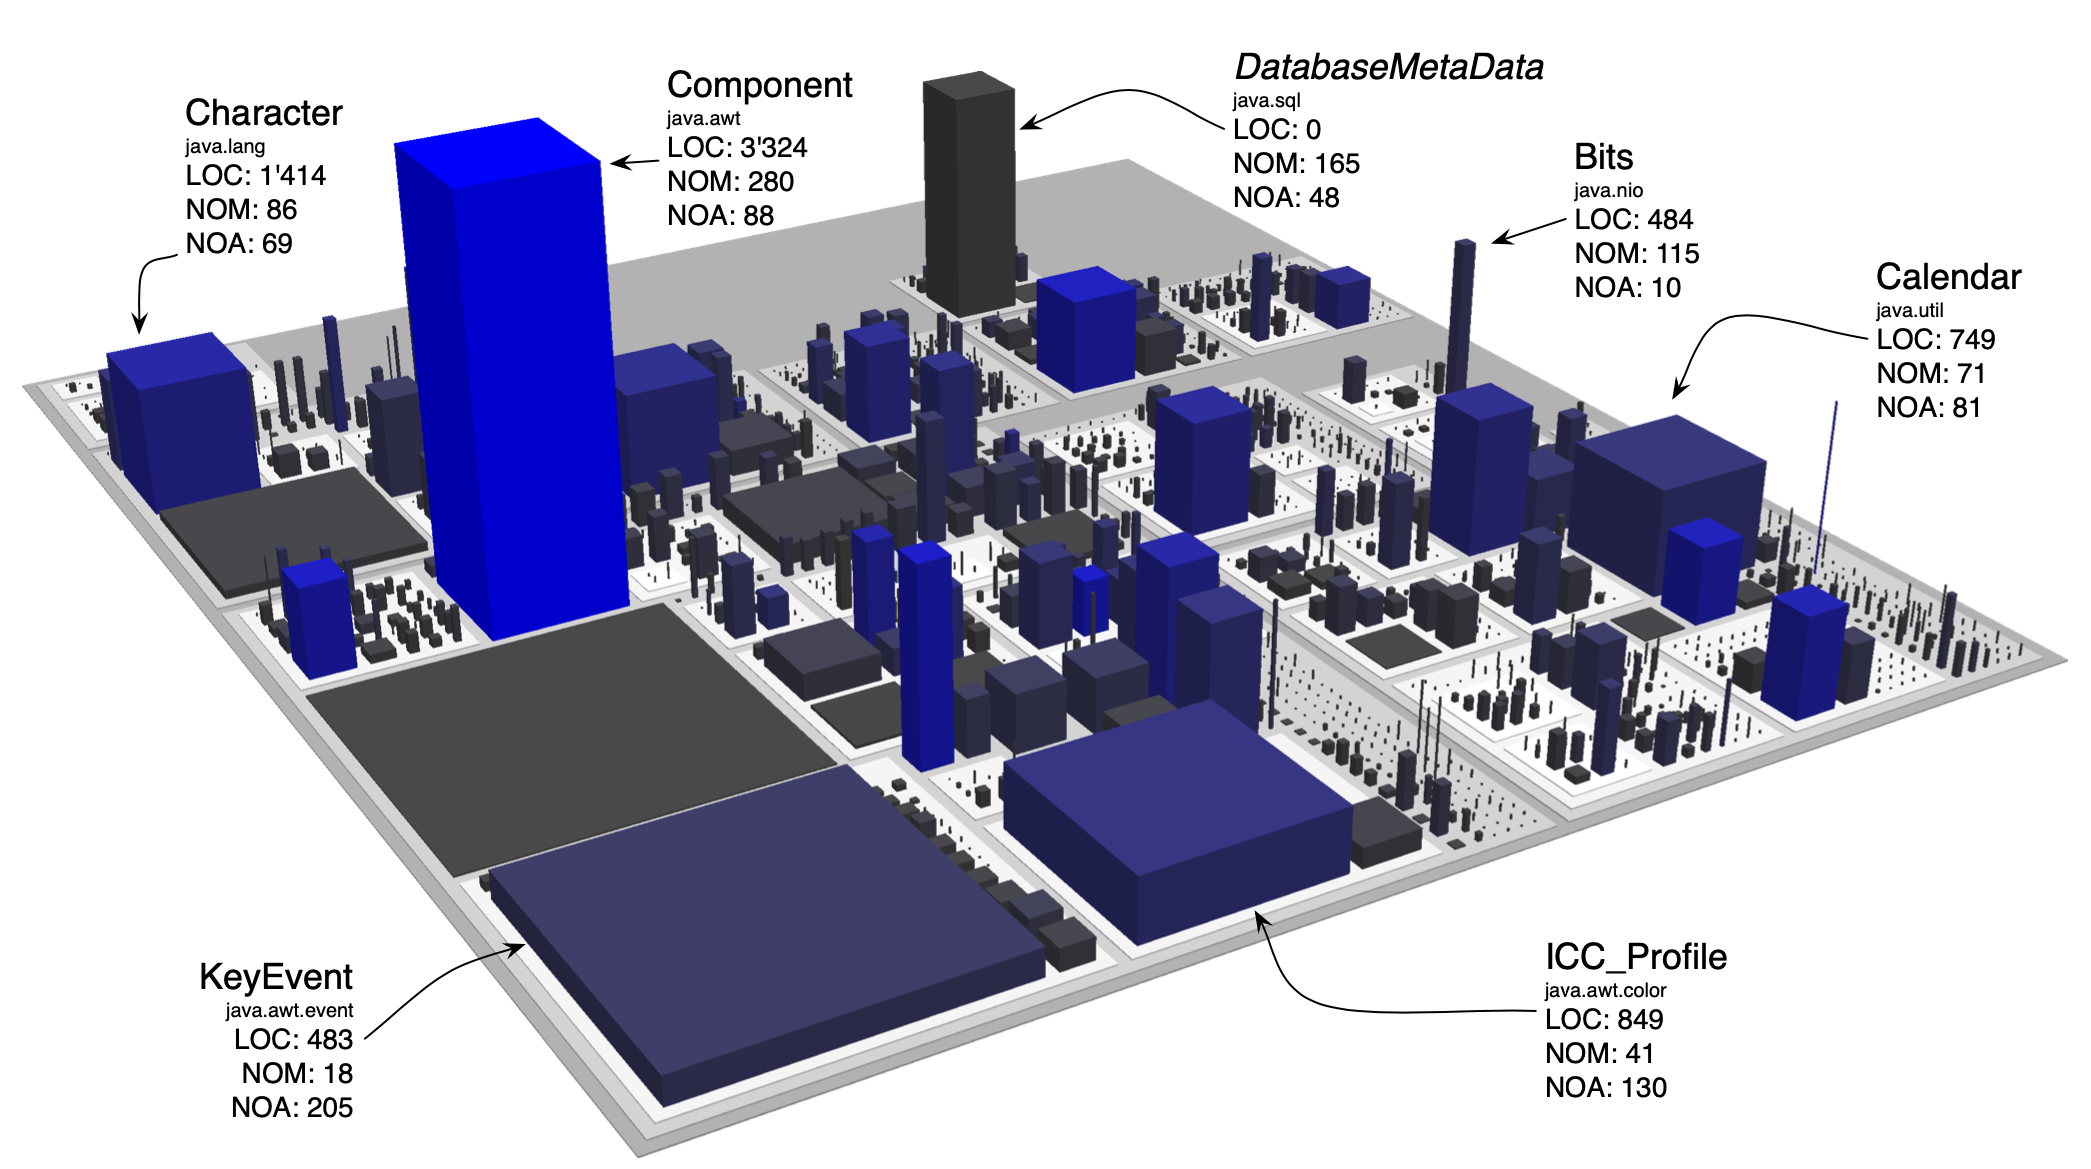
\includegraphics[width=\textwidth]{CodeCity.png}